\documentclass[12pt, a4paper]{article}
\usepackage[utf8]{inputenc}
\usepackage{amsmath} 
\usepackage{amssymb}
\usepackage{listings}
\usepackage{graphicx}
\usepackage{float}
\usepackage[dvipsnames]{xcolor}
\PassOptionsToPackage{hyphens}{url}
\usepackage{hyperref}

\begin{document}

\section{Implementation}

\subsection{Data Collection}

There is no historical data for bus arrival times available online, so all the data that I will use to train and test my models has to be manually collected. \\

The following bus routes were chosen to collect data from: 452, 9, 52, 267, 277, 7, 6, 14, 35, 37, 69, 328. Of these routes, the 52, 6, 14, 37 and 69 bus routes are twenty four hour bus routes and the 267, 277, 37 and 69 bus routes do not travel through Zone 1. This allows there to be variety in the travel routes, traffic conditions and times of travel and so the data collected is not heavily biased towards particular areas of London. There is also some overlap in stops between the bus routes, for example the 52 to Victoria and the 452 to Vauxhall have a 23 stop (and therefore, also route) overlap from "Station Terrace" to  "Knightsbridge Station /\ Harrods". This ensures information on journey times between stops doesn't rely on data from just one bus route.

\textbf{1) Call Countdown API}: The Countdown API is called for each stop on the specified route and returns a JSON of the form [[URA array],[Prediction Array]]. An example is shown in Figure \ref{fig:countdown-response}, where Countdown was called for bus route 9, stop code 490010357F (commonly known as "North End Road"). 

\begin{figure}[H]
\begin{center}
    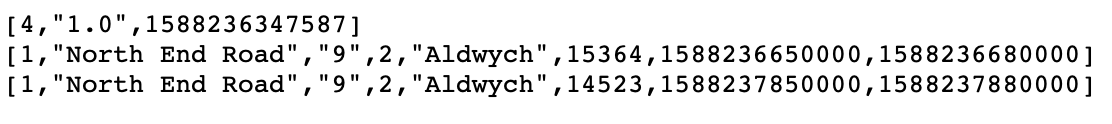
\includegraphics[keepaspectratio, width=14cm]{Images/Countdown-result.png}
    \caption{Countdown API response}
    \label{fig:countdown-response}
\end{center}
\end{figure}

Each item in the \textit{Prediction} array corresponds to each of the response items as stated previously. This data is then converted into a list of dictionaries, where each dictionary represents a single vehicle. The format of each dictionary is as below:

\begin{lstlisting}
    vehicle_info = {
                "vehicle_id": vehicle_id,
                "bus_stop_name": bus_stop_name,
                "direction": direction,
                "expected_arrival": eta,
                "time_of_req": time_of_request,
                "arrived": False
            }
\end{lstlisting}

In the dictionary, the \texttt{vehicle\_id}, \texttt{bus\_stop\_name} and \texttt{direction} are strings. The \texttt{expected\_arrival} and \texttt{time\_of\_req} are Python \texttt{Datetime} objects and \texttt{arrived} is a boolean. \\

\textbf{2) Update the estimated arrival time of a bus}: For each of the items returned in the API call, check if the vehicle corresponds to one already in the \texttt{bus\_information\_route} table. If it already exists, then update its expected arrival time, otherwise, it is a new vehicle to track and add to the table. \\

\textbf{3) Check if the bus has arrived or not}:  If the current time is after the predicted arrival time of the bus, then it is classified as 'due'. If the current time is 5 minutes after the predicted arrival time of the bus, then it is classified as 'arrived'. \\

\textbf{4) Write to the relevant database} Once a bus is classified as 'arrived', remove it from the \texttt{bus\_information\_route} table and add it to the \texttt{bus\_arrivals\_route} table. When adding to the \texttt{bus\_arrivals\_route} table, check to see if on this day this particular vehicle is already in the table. It is necessary to check this because each vehicle will complete the bus route more than once per day, and therefore, the current trip number has to be kept track of too. \\

\textbf{Data stores}

\begin{itemize}
    \item \texttt{valid\_stop\_ids\_route} stores the list of valid stop ids and its respective plain English name for that particular route. 
    \item \texttt{bus\_information\_route} stores information on buses that haven't arrived yet for a particular route.
    \item \texttt{bus\_arrivals\_route} stores information on all buses that have arrived for this route. 
\end{itemize}

\begin{figure}[H]
\begin{center}
    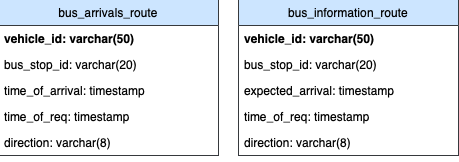
\includegraphics[keepaspectratio, width=10cm]{Images/database-diagrams.png}
    \caption{Databases}
    \label{fig:databases}
\end{center}
\end{figure}

\subsection{Data Analytics}

Clustering, graphs, exploring the data

\begin{figure}[H]
\begin{center}
    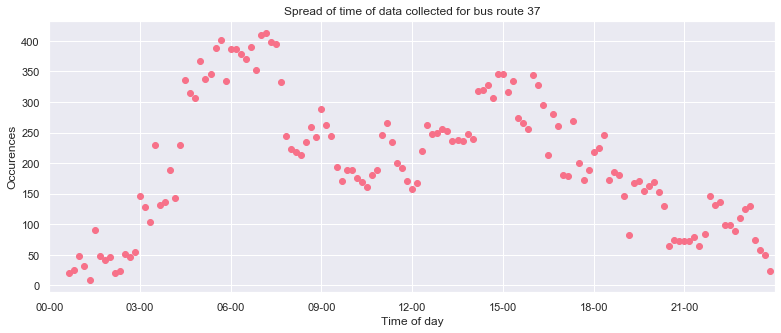
\includegraphics[keepaspectratio, width=15cm]{Images/spread-of-buses-37.png}
    \caption{Number of buses during the day for route 37}
    \label{fig:spread-of-buses-over-day}
\end{center}
\end{figure}

\subsection{Historical Models}

\begin{figure}[H]
\begin{center}
    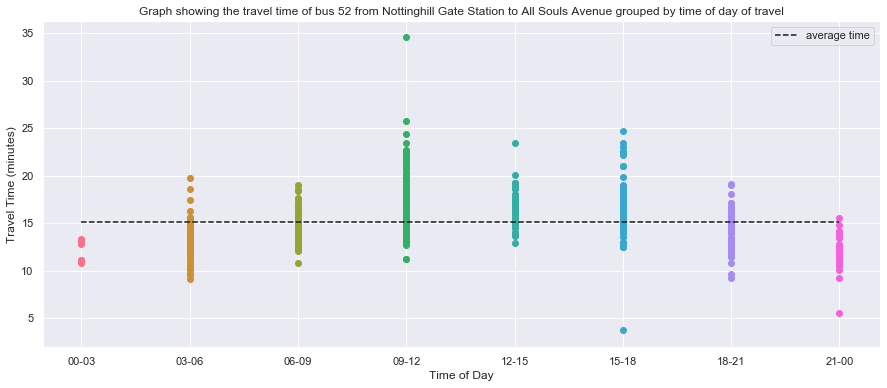
\includegraphics[keepaspectratio, width=15cm]{Images/delay-by-time-of-day-52.png}
    \caption{Delay by time of day}
    \label{fig:databases}
\end{center}
\end{figure}

\begin{figure}[H]
\begin{center}
    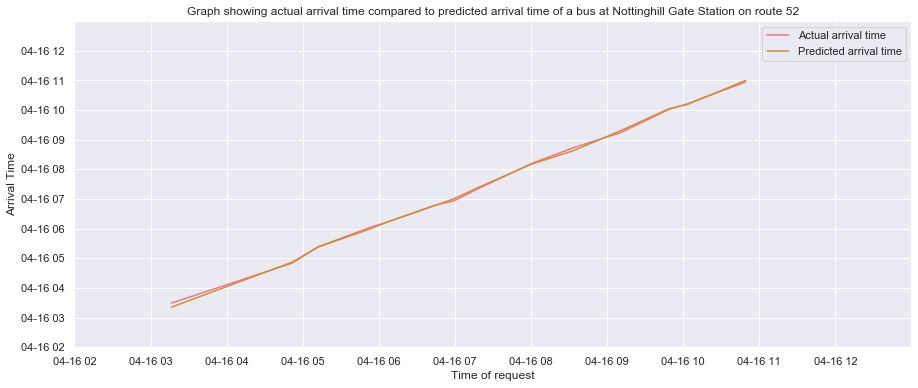
\includegraphics[keepaspectratio, width=15cm]{Images/historical-pred-actual-52.png}
    \caption{Bus 52}
    \label{fig:historical-pred-actual}
\end{center}
\end{figure}

\subsection{Regression Models}

\subsection{Neural Network Models}

\clearpage

\end{document}